% f2015hbw_q15_mountain.tex — 2015 年高考数学·湖北卷·文科 第 15 题（山高示意图）
%
% 【来源】`.work/phase3-b20/source/2015湖北文.pdf`（SHA-256
%   801e73338b6c4c747cc76b14e167d590a34e0b5a13a47719e5ee6cd4337e4cd2），
%   第 1 页（合订本页 953）；内容对象 5/7/9/…/19。逐路径实测见
%   `.work/phase3-b20/figure-inventory.md`。
%
% 【坐标口径】源 PDF 用户空间（原点左下、y 向上）。本图本地坐标
%   (x, y) = (x_page − 517.62, y_page − 56.892)，1 单位 = 1 TeX pt。
%   路径坐标逐点照录内容流（含三次贝塞尔控制点）。
%
% 元素计数：12 条路径（两条水平线、山体折线、CD 竖线、BC 线、虚线视线、2 车体＋4 车轮）＋4 个标签
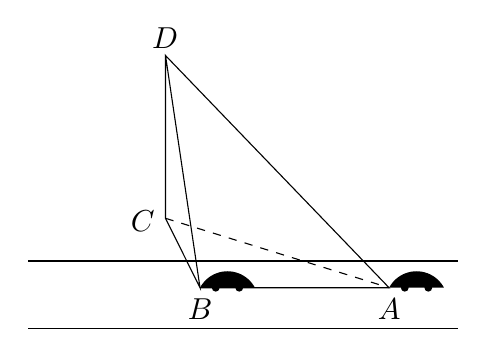
\begin{tikzpicture}[x=1pt, y=1pt,
    every node/.style={inner sep=0pt, font=\fontsize{10.5pt}{12.6pt}\selectfont}]
  \draw[line width=0.398pt] (-0.0004,24.4589)   -- (155.3116,24.4589);
  \draw[line width=0.398pt] (-0.0004,-0.0002)   -- (155.3116,-0.0002);
  \draw[line width=0.398pt] (49.6065,98.7276)   -- (49.6065,39.9076)   -- (62.0795,14.8206)   -- (49.6065,98.7276)   -- (130.3945,14.8206)   -- (62.0795,14.8206);
  \draw[line width=0.398pt] (49.6065,98.7276)   -- (49.6065,39.9076);
  \draw[line width=0.398pt] (62.0792,14.8209)   -- (130.3952,14.8209);
  \draw[line width=0.398pt, dash pattern=on 2.989pt off 2.989pt, dash phase=0.0pt] (49.6065,39.9079)   -- (130.3945,14.8209);
  \fill[line width=0.398pt] (150.2373,14.8207)   .. controls (150.2373,14.8207) and (149.8743,15.4567) .. (149.7213,15.6917)   .. controls (149.5673,15.9267) and (149.3023,16.2927) .. (149.1283,16.5127)   .. controls (148.9543,16.7327) and (148.6583,17.0737) .. (148.4643,17.2767)   .. controls (148.2713,17.4797) and (147.9463,17.7927) .. (147.7353,17.9787)   .. controls (147.5243,18.1637) and (147.1723,18.4457) .. (146.9453,18.6117)   .. controls (146.7183,18.7767) and (146.3423,19.0267) .. (146.1013,19.1707)   .. controls (145.8613,19.3147) and (145.4633,19.5297) .. (145.2113,19.6517)   .. controls (144.9583,19.7737) and (144.5433,19.9517) .. (144.2813,20.0507)   .. controls (144.0183,20.1497) and (143.5893,20.2897) .. (143.3183,20.3647)   .. controls (143.0483,20.4397) and (142.6083,20.5407) .. (142.3313,20.5907)   .. controls (142.0553,20.6417) and (141.6083,20.7027) .. (141.3293,20.7277)   .. controls (141.0493,20.7527) and (140.5983,20.7737) .. (140.3173,20.7737)   .. controls (140.0373,20.7737) and (139.5863,20.7527) .. (139.3073,20.7277)   .. controls (139.0273,20.7027) and (138.5803,20.6417) .. (138.3043,20.5917)   .. controls (138.0273,20.5417) and (137.5873,20.4407) .. (137.3173,20.3657)   .. controls (137.0463,20.2907) and (136.6173,20.1507) .. (136.3543,20.0527)   .. controls (136.0923,19.9537) and (135.6773,19.7757) .. (135.4243,19.6537)   .. controls (135.1713,19.5307) and (134.7743,19.3167) .. (134.5333,19.1727)   .. controls (134.2923,19.0287) and (133.9163,18.7787) .. (133.6893,18.6137)   .. controls (133.4633,18.4477) and (133.1103,18.1657) .. (132.8993,17.9807)   .. controls (132.6883,17.7957) and (132.3633,17.4827) .. (132.1693,17.2787)   .. controls (131.9763,17.0757) and (131.6803,16.7347) .. (131.5063,16.5147)   .. controls (131.3313,16.2947) and (131.0673,15.9287) .. (130.9133,15.6947)   .. controls (130.7593,15.4597) and (130.3963,14.8237) .. (130.3963,14.8237);
  \fill[line width=0.398pt] (81.9216,14.8207)   .. controls (81.9216,14.8207) and (81.5586,15.4567) .. (81.4056,15.6917)   .. controls (81.2516,15.9267) and (80.9866,16.2927) .. (80.8126,16.5127)   .. controls (80.6386,16.7327) and (80.3426,17.0737) .. (80.1486,17.2767)   .. controls (79.9556,17.4797) and (79.6306,17.7927) .. (79.4196,17.9787)   .. controls (79.2086,18.1637) and (78.8566,18.4457) .. (78.6296,18.6117)   .. controls (78.4026,18.7767) and (78.0266,19.0267) .. (77.7866,19.1707)   .. controls (77.5456,19.3147) and (77.1476,19.5297) .. (76.8956,19.6517)   .. controls (76.6426,19.7737) and (76.2276,19.9517) .. (75.9656,20.0507)   .. controls (75.7026,20.1497) and (75.2736,20.2897) .. (75.0026,20.3647)   .. controls (74.7326,20.4397) and (74.2926,20.5407) .. (74.0166,20.5907)   .. controls (73.7396,20.6417) and (73.2926,20.7027) .. (73.0136,20.7277)   .. controls (72.7336,20.7527) and (72.2826,20.7737) .. (72.0016,20.7737)   .. controls (71.7216,20.7737) and (71.2706,20.7527) .. (70.9916,20.7277)   .. controls (70.7116,20.7027) and (70.2646,20.6417) .. (69.9886,20.5917)   .. controls (69.7116,20.5417) and (69.2716,20.4407) .. (69.0016,20.3657)   .. controls (68.7306,20.2907) and (68.3016,20.1507) .. (68.0386,20.0527)   .. controls (67.7766,19.9537) and (67.3616,19.7757) .. (67.1086,19.6537)   .. controls (66.8556,19.5307) and (66.4586,19.3167) .. (66.2176,19.1727)   .. controls (65.9766,19.0287) and (65.6006,18.7787) .. (65.3736,18.6137)   .. controls (65.1476,18.4477) and (64.7946,18.1657) .. (64.5836,17.9807)   .. controls (64.3736,17.7957) and (64.0476,17.4827) .. (63.8536,17.2787)   .. controls (63.6606,17.0757) and (63.3646,16.7347) .. (63.1906,16.5147)   .. controls (63.0156,16.2947) and (62.7516,15.9287) .. (62.5976,15.6947)   .. controls (62.4436,15.4597) and (62.0816,14.8237) .. (62.0816,14.8237);
  \fill[line width=0.398pt] (137.4817,14.8209)   .. controls (137.4817,15.6039) and (136.8467,16.2379) .. (136.0647,16.2379)   .. controls (135.2817,16.2379) and (134.6467,15.6039) .. (134.6467,14.8209)   .. controls (134.6467,14.0379) and (135.2817,13.4039) .. (136.0647,13.4039)   .. controls (136.8467,13.4039) and (137.4817,14.0379) .. (137.4817,14.8209)   -- cycle;
  \fill[line width=0.398pt] (145.9857,14.8209)   .. controls (145.9857,15.6039) and (145.3507,16.2379) .. (144.5687,16.2379)   .. controls (143.7857,16.2379) and (143.1507,15.6039) .. (143.1507,14.8209)   .. controls (143.1507,14.0379) and (143.7857,13.4039) .. (144.5687,13.4039)   .. controls (145.3507,13.4039) and (145.9857,14.0379) .. (145.9857,14.8209)   -- cycle;
  \fill[line width=0.398pt] (69.1658,14.8209)   .. controls (69.1658,15.6039) and (68.5308,16.2379) .. (67.7488,16.2379)   .. controls (66.9658,16.2379) and (66.3308,15.6039) .. (66.3308,14.8209)   .. controls (66.3308,14.0379) and (66.9658,13.4039) .. (67.7488,13.4039)   .. controls (68.5308,13.4039) and (69.1658,14.0379) .. (69.1658,14.8209)   -- cycle;
  \fill[line width=0.398pt] (77.6700,14.8209)   .. controls (77.6700,15.6039) and (77.0350,16.2379) .. (76.2530,16.2379)   .. controls (75.4700,16.2379) and (74.8350,15.6039) .. (74.8350,14.8209)   .. controls (74.8350,14.0379) and (75.4700,13.4039) .. (76.2530,13.4039)   .. controls (77.0350,13.4039) and (77.6700,14.0379) .. (77.6700,14.8209)   -- cycle;

  \node[anchor=center] at (49.430,105.048) {$D$};  % 源中心 (567.05,161.94)
  \node[anchor=center] at (41.430,38.948) {$C$};  % 源中心 (559.05,95.84)
  \node[anchor=center] at (62.080,7.148) {$B$};  % 源中心 (579.70,64.04)
  \node[anchor=center] at (130.430,7.148) {$A$};  % 源中心 (648.05,64.04)

\end{tikzpicture}
%
% 【自验结果】
%   探针：latexmk -pdfxe（待跑）。
